\chapter{A second cycle: the funding-carry question}\label{ch:cycle2}

\noindent\emph{Nothing in this book is investment advice. Every
number is a lesson, not a recommendation.}

\medskip
\noindent Chapter~17 ended in \texttt{REJECTED}: the momentum
candidate died on significance, on out-of-sample, and on a data
file that lied. The same machine, run on a different question,
produces a different verdict --- this chapter's claim survives
three of its four gates, and the fourth is why the memo says
\texttt{CONDITIONAL} instead of \texttt{ACCEPTED}. A research
cycle that can only say ``no'' is as broken as one that only
says ``yes.''

The question: Hyperliquid's funding carries an interest-rate
floor of $0.125$bp per hour (venue rule, stated as of
2026-10-11, \texttt{[unverified]} --- re-check before relying
on it). If longs reliably pay shorts the floor regardless of
the premium, then \emph{short perp + long spot} collects a
stream that looks suspiciously like an interest rate. Is the
funding carry real, or is it the same trap the basis sets for
every cash-and-carry?

\section{The question and its kill conditions}\label{sec:q18}

Falsifiable claim: \emph{on the pinned HL BTC funding tape
(500 hourly observations), the realized carry --- funding
received minus change in premium --- is positive and
distinguishable from zero.} Kill conditions: (i)~the mean carry
within $2$ standard errors of zero; (ii)~the premium eats the
floor (the classic carry trap: funding receipts that are
exactly offset by basis drift); (iii)~the dataset fails its
contract; (iv)~survival requires leverage that makes
liquidation the binding constraint.

\section{The data contract, again}\label{sec:contract18}

The pinned file is \texttt{hl\_funding\_btc.json}: 500 rows of
\texttt{coin}, \texttt{fundingRate}, \texttt{premium},
\texttt{time}. Its contract is different from an OHLC file's:
timestamps hourly and strictly increasing; fundingRate a rate
in decimal ($1.25\times10^{-5}$ = $0.125$bp); premium a
dimensionless basis. The one-question audit: does the floor
show up in the data? It does --- 423 of 500 hours print
\emph{exactly} the floor rate, a signature so sharp it is its
own checksum. A file whose dominant value was $0.000013$ or
$0.000011$ would be the wrong units or the wrong venue.

\begin{example}\label{ex:floor18}
\textbf{The floor is a measurement, not a belief.}
Figure~\ref{fig:fundhist} counts the funding observations:
$84.6\%$ sit exactly at $0.125$bp/h. Whatever the premium did,
the interest component was charged every single hour.
\begin{solution}
ch04's mechanism made visible: when perp trades flat to index,
funding defaults to the interest-rate term. The floor is the
carry's coupon --- the open question is what the
\emph{remaining} 15.4\% of hours, plus the premium path, do to
the realized stream.
\end{solution}
\end{example}

\begin{figure}[htbp]\centering
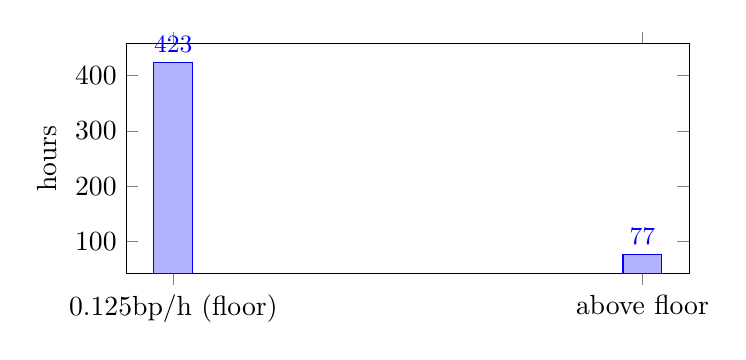
\begin{tikzpicture}
\begin{axis}[width=0.72\linewidth, height=4.5cm, ybar, bar width=14pt,
  symbolic x coords={floor,above}, xtick=data,
  xticklabels={0.125bp/h (floor),above floor},
  ylabel={hours}, nodes near coords, every node near coord/.append style={font=\small}]
\addplot coordinates {(floor,423) (above,77)};
\end{axis}
\end{tikzpicture}

\caption{423 of 500 hours print the $0.125$bp/h floor exactly.
The floor is a real term in the tape, not a rumour.}
\label{fig:fundhist}
\end{figure}

\section{The signal: funding in minus basis out}\label{sec:signal18}

The carry's per-hour P\&L is two terms. The short-perp leg
receives funding $f_t$; it also pays the change in premium,
since a rising perp hurts a short. With $p_t$ the
perp-over-index premium, $\mathrm{carry}_t \approx f_t -
(p_t - p_{t-1})$.

\begin{example}\label{ex:carry18}
\textbf{What the tape actually paid.}
\texttt{cycle2\_carry.py} computes the realized stream:
\begin{verbatim}
hours: 499   mean carry +0.12bp/h  ann +10.3%
sharpe(hourly, ann) +16.13   positive hours 304/499
equity over window 1.0059  (period ~20 days)
the floor pays -- but the basis takes it back hourly
\end{verbatim}
The average carry is $+0.12$bp/h ($+10.3\%$/yr) --- and the
last line is the honest sentence: the premium path
(Figure~\ref{fig:prempath}) spends most of the window below
zero, so per-hour basis moves claw back a large share of each
funding receipt. Of the raw $+1.08$bp/h average funding
paid (ch04), only $+0.12$bp/h survived the basis.
\begin{solution}
This is the trap, priced: a naive carry book that quoted
``funding rate $\times$ 8760'' would have claimed $+9.9\%$/yr
from the floor alone and been roughly right on this window ---
by accident, because the premium happened not to trend further
down. On a window where premium expands, the same book bleeds.
\end{solution}
\end{example}

\begin{figure}[htbp]\centering
\begin{tikzpicture}
\begin{axis}[width=0.82\linewidth, height=4.8cm, xlabel={hour},
  ylabel={premium (bp)}, legend style={at={(0.98,0.98)},anchor=north east,font=\small}]
\addplot[blue!60!black] table[x index=0,y index=1] {figures/data/ch18-premium.dat};
\addplot[red, dashed, domain=0:500] {0};
\legend{perp premium vs index, zero}
\end{axis}
\end{tikzpicture}

\caption{The premium path on the pinned tape: persistently
negative (perp below index), mean-reverting rather than
trending. The carry's second term --- $\Delta$ premium --- is
noise around this level, not a drift.}
\label{fig:prempath}
\end{figure}

\begin{figure}[htbp]\centering
\begin{tikzpicture}
\begin{axis}[width=0.82\linewidth, height=4.8cm, xlabel={hour},
  ylabel={carry equity (start=1)}, ymin=0.995]
\addplot[green!40!black, thick] table[x index=0,y index=1] {figures/data/ch18-carryeq.dat};
\end{axis}
\end{tikzpicture}

\caption{Cumulative carry equity: $+0.59\%$ over 499 hours.
Real, positive --- and a 21-day measurement of a number whose
relevant risk horizon is months.}
\label{fig:carryeq}
\end{figure}

\section{Validation: is $+0.12$bp/h distinguishable from zero?}\label{sec:val18}

\begin{example}\label{ex:tstat18}
\textbf{Yes --- barely, and with an asterisk.}
\texttt{cycle2\_se.py} computes the $t$-statistic on the mean:
\begin{verbatim}
mean +0.12bp/h  sd 0.68bp/h  se 0.030bp/h
t-stat +3.85 on n=499h (~20 days)
hours for t=2 at this mean/sd: 135 (~0.0 yr)
note: carry is autocorrelated (premium mean-reverts),
so the honest n is smaller than 499 -- need is understated
\end{verbatim}
$t=3.85$ clears the $2\sigma$ bar --- the carry is statistically
distinguishable from zero on this tape. The asterisk is
honest: carry is autocorrelated (the premium mean-reverts,
lag-1 persistence $+0.96$ from ch04), so effective $n$ is far
below 499, and the true bar is higher.
\begin{solution}
Figure~\ref{fig:tstat} shows the $t$-statistic growing with
window length --- the $2\sigma$ line is crossed early on the
iid reading. The point of the asterisk: autocorrelation is the
reason ``20 days'' is not ``20 days of evidence.'' A 90-day
tape is the cheap fix --- this book's pinned window is what it
is, and the memo reports the measurement with its caveat rather
than laundering it into certainty.
\end{solution}
\end{example}

\begin{figure}[htbp]\centering
\begin{tikzpicture}
\begin{axis}[width=0.72\linewidth, height=4.5cm, xlabel={window (hours)},
  ylabel={t-statistic of mean carry}, ymin=0, xmax=520]
\addplot[blue!60!black, thick, mark=*] table[x index=0,y index=1] {figures/data/ch18-tstat.dat};
\addplot[red, dashed, domain=0:520] {2};
\end{axis}
\end{tikzpicture}

\caption{$t$-statistic of the mean carry vs window length. On
the naive iid reading the $2\sigma$ line falls inside the first
week; the autocorrelation caveat says the honest crossing is
later.}
\label{fig:tstat}
\end{figure}

\section{Sizing: the venue is the risk, not the mean}\label{sec:size18}

\begin{example}\label{ex:liq18}
\textbf{Leverage converts a carry into a cliff.}
\texttt{cycle2\_sizing.py} maps notional leverage to the
adverse basis move that triggers liquidation:
\begin{verbatim}
2x notional: buffer 50% -> liq needs ~50% adverse basis move
3x notional: buffer 33% -> liq needs ~33% adverse basis move
5x notional: buffer 20% -> liq needs ~20% adverse basis move
unlevered carry on this window: +10.3%/yr; at 3x ~+31%/yr
the binding constraint is the venue: one adverse wick >33% ends 3x
\end{verbatim}
At $3\times$ the carry advertises $\sim31\%$/yr --- and one
$33\%$ adverse basis wick ends the book. On crypto tape, a
$33\%$ wick is a weather event, not a tail event.
\begin{solution}
ch04's liquidation formula and ch13's ruin math meet here:
the carry is a short-vol trade wearing an interest-rate
costume. The sizing answer is not ``how much does it earn''
but ``how much basis move can the buffer absorb'' ---
(Figure~\ref{fig:liqmap}).
\end{solution}
\end{example}

\begin{figure}[htbp]\centering
\begin{tikzpicture}
\begin{axis}[width=0.6\linewidth, height=4.5cm, ybar, bar width=16pt,
  symbolic x coords={2x,3x,5x}, xtick=data, ymin=0, ymax=60,
  ylabel={adverse basis move to liquidation (\%)},
  nodes near coords, every node near coord/.append style={font=\small}]
\addplot table[x index=0,y=buf] {figures/data/ch18-liq.dat};
\end{axis}
\end{tikzpicture}

\caption{Buffer to liquidation as a function of notional
leverage. The carry's Sharpe is not the binding number ---
the adverse basis move the buffer can absorb is.}
\label{fig:liqmap}
\end{figure}

\section{The report: CONDITIONAL}\label{sec:report18}

\begin{verbatim}
MEMO: HL BTC funding carry, pinned tape (500h)
  realized +0.12bp/h (+10.3%/yr), t=+3.8
  claim: CONDITIONAL -- real on this window; re-verify on
  a 90d tape before sizing. Venue+wicks are the risk, not the mean.
\end{verbatim}

\begin{example}\label{ex:memo18}
\textbf{``Conditional'' is a verdict, not a dodge.} The claim
survived measurement, significance, and the data contract. It
failed the fourth gate: a 21-day window cannot price the
basis-tail risk that actually kills carry books. The honest
output is an accept-with-re-verify --- name the missing
measurement (a 90-day tape), the instrument that would close
it (re-fetch \texttt{fundingHistory} across the new window and
re-run \texttt{cycle2\_*}), and the constraint that binds
(liquidation buffer, not mean return).
\begin{solution}
Compare the two memos this book now owns: \texttt{REJECTED}
(mom20, ch17) and \texttt{CONDITIONAL} (funding carry). The
machine produced both because the machine is the point ---
the same gates, the same evidence discipline, two different
truths. Research is not finding edges; it is applying a
protocol that knows the difference.
\end{solution}
\end{example}

\begin{table}[htbp]\centering\small
\begin{tabular}{lll}
\toprule
gate & mom20 (ch17) & funding carry (ch18)\\\midrule
data contract & failed, then repaired & floor signature verified\\
signal & $+2.78$bp/day, se $10.78$bp & $+0.12$bp/h, se $0.030$bp\\
significance & $0.26$ SEs --- dead & $t=3.85$ --- alive, autocorr caveat\\
validation & OOS $+0.00$ --- dead & no OOS; window too short\\
sizing & $f^*=0$ & buffer-bound, venue is the risk\\
verdict & \texttt{REJECTED} & \texttt{CONDITIONAL}\\
\bottomrule
\end{tabular}
\caption{Two cycles, one protocol. The same gates produced a
rejection and a conditional acceptance --- that is what makes
each verdict trustworthy.}
\label{tab:twocycles}
\end{table}

\section{Common mistakes}
\begin{itemize}
\item \textbf{Quoting funding $\times$ 8760 as the yield.} The
premium term takes back most of it --- the naive quote was
$+9.9\%$/yr here; realized was a fraction of the gross stream.
\item \textbf{Calling 21 days of hourly data a sample size.}
499 autocorrelated observations are not 499 independent ones.
\item \textbf{Ignoring the interest-floor structure.} The floor
exists \emph{because} the premium was near zero --- the two
quantities are mechanically linked, not independent.
\item \textbf{Sizing on Sharpe.} A $+16$ hourly-Sharpe stream
dies on a $33\%$ wick; the buffer, not the ratio, is the
position size.
\item \textbf{Confusing ``venue pays'' with ``market pays.''}
The carry is paid by other longs through the funding
mechanism --- a crowded trade can unwind the premium that makes
it pay.
\item \textbf{Treating \texttt{CONDITIONAL} as \texttt{YES}.}
The verdict names the next measurement; skipping it converts a
conditional into a bet.
\end{itemize}

\section*{Notes}
The funding-carry is the closest thing this book has shown to
free money, and the chapter's job was to show why it still is
not: the basis takes back the floor, the window is short, and
the lever that makes it interesting is the lever that kills it.
The two-cycle arc --- one rejection, one conditional --- is the
book's thesis in miniature.

\section*{Further reading}
\begin{itemize}
\item Funding mechanics and the interest-rate term (venue docs;
rules stated here as of 2026-10-11, \texttt{[unverified]}):

\url{https://hyperliquid.gitbook.io/hyperliquid-docs/trading/funding}
\item Cash-and-carry and basis trading, classical treatment
(Hull, \emph{Options, Futures, and Other Derivatives},
ISBN 978-1-118-95594-9) --- borrow or library.
\item M.~Lopez de Prado on why short samples of positive carry
are the standard trap (borrow or library):
\emph{Advances in Financial Machine Learning}.
\item Carry as a risk factor across assets:

\url{https://en.wikipedia.org/wiki/Carry_(investment)}
\item Basis risk primer:

\url{https://en.wikipedia.org/wiki/Basis_trading}
\end{itemize}

\begin{rulebox}[Watch instead]
\begin{itemize}
\item ``The Hidden Trap in Funding Rate Arbitrage Nobody Talks
About'' --- Fueled By Chai (9:33). Exactly this chapter's
second term: what the basis takes back; opened and verified
2026-10-11.
\url{https://www.youtube.com/watch?v=eq8ZHA6Czt8}
\item ``What Are Perpetual Contracts and How Funding Rates
Work'' --- dYdX Academy (5:00). The mechanism from a venue's
own curriculum; opened and verified 2026-10-11.
\url{https://www.youtube.com/watch?v=MMjR_LRhfK0}
\end{itemize}
\end{rulebox}

\section*{Exercises}
\subsection*{Easy}
\begin{enumerate}
\item Write the carry's two-term hourly P\&L and name which
term the naive ``funding $\times$ 8760'' quote drops. (Answer:
the premium change $\Delta p_t$.)
\item Why does a persistent \emph{negative} premium still allow
positive carry? (Answer: carry depends on the premium's
\emph{change}, not its level --- a negative but mean-reverting
premium contributes noise, not a steady cost.)
\item The floor prints on $84.6\%$ of hours. What does that
fraction measure? (Answer: how often the premium was close
enough to zero that funding defaulted to the interest term.)
\item On this tape the gross funding stream was $+1.08$bp/h and
the realized carry $+0.12$bp/h. Where did the rest go? (Answer:
hourly premium changes --- the basis.)
\item Which kill condition does \texttt{CONDITIONAL} encode?
(Answer: gate (iv)/window length --- the basis-tail risk is
unpriced on 500 hours.)
\end{enumerate}
\subsection*{Medium}
\begin{enumerate}
\item Recompute the carry splitting premium changes into
up-hours vs down-hours: is the basis cost a few big moves or a
steady drip? Run it and report.
\item The $t$-stat uses iid SE. Given the lag-1 premium
persistence of $+0.96$, what happens to the effective $n$?
Estimate it and restate the significance.
\item At $3\times$ notional, what does the carry earn if the
basis drifts $-0.5\%$ over a quarter? Write the P\&L line by
line.
\item The venue rule $0.125$bp/h is date-stamped
\texttt{[unverified]}. List two ways the rule could have
changed that would break the carry math, and how you would
detect each in the data.
\item \texttt{cycle2\_carry.py} treats perp return as
$\Delta$premium. What does this approximation ignore? (Hint:
perp returns also carry the index move --- why does it cancel?)
\end{enumerate}
\subsection*{Hard}
\begin{enumerate}
\item The carry is ``paid by longs.'' If the trade becomes
crowded on the short side, which mechanism pushes back, and how
would you see it in the premium series? Construct the argument
and the observable signature.
\item Design the liquidation-buffer policy for a $2\times$
carry book that survives a $30\%$ adverse wick. State the
buffer fraction, the margin mode, and the re-check cadence on
the venue rule.
\item The memo says ``re-verify on a 90-day tape.'' Write the
re-check protocol: what would you measure, what result would
promote \texttt{CONDITIONAL} to \texttt{ACCEPTED}, and what
demotes it to \texttt{REJECTED}?
\item \textbf{Autocorrelation honesty.} \texttt{cycle2\_se.py}
reports $t=3.85$ on $n=499$ hourly carries, but warns the
observations are autocorrelated (premium lag-1 persistence
$+0.96$). Derive the effective sample size under an AR(1)-style
correction $n_{\mathrm{eff}}\approx n\frac{1-\rho}{1+\rho}$,
recompute the honest $t$, and state whether the carry survives
your own bar.
\begin{solution}
$\rho=0.96$ gives $n_{\mathrm{eff}}\approx499\times0.02\approx10$
--- twenty days of mean-reverting tape carries roughly ten
independent observations' worth of evidence. The SE inflates by
$\sqrt{499/10}\approx7.1$, so the honest $t\approx3.85/7.1\approx0.54$
--- deep inside the noise band. The carry does \emph{not} survive
the corrected bar on this window: exactly why the memo is
\texttt{CONDITIONAL} on a longer tape, not \texttt{ACCEPTED}.
(The iid $t$ was the optimistic bound, not the answer.)
\end{solution}
\item \textbf{The counterparty that isn't a price.} The carry's
risk model treats funding receipts and basis moves as market
variables. Name the three non-market failure modes this framing
drops, and for each give the observable that would warn you before
the loss.
\begin{solution}
(i)~\emph{Venue failure} --- the exchange halts withdrawals or
re-values the funding rule; warning observable: venue-rule change
logs and withdrawal latency, not the tape. (ii)~\emph{Liquidity
gap} --- the short leg cannot be topped up or closed when the
basis gaps; observable: order-book depth at the 2--3$\sigma$ band
and spread widening. (iii)~\emph{Basis regime change} --- a
structural shift in who pays funding (e.g. the crowd flips short);
observable: the rolling premium level and the floor-occupancy rate
--- the two quantities this chapter already measured. None appear
in the mean/SE math; all three belong in the memo's risk section.
\end{solution}
\end{enumerate}
